%%\usepackage[top=2cm,bottom=2cm,left=1cm,right=1cm]{geometry}


\begin{titlepage}
     \begin{center}
	
\includegraphics[width=0.09\textwidth]{UNAM}\Large Universidad Nacional Autónoma de México
        	
\includegraphics[width=0.09\textwidth]{FI}\\[1cm]
        \Large Facultad de Ingeniería\\[1cm]
       % \Large División de Ciencias Básicas\\[1cm]
         \Large Laboratorio de Fundamentos de Control(6655)\\[1cm]
         %la clave antes era:4314
         \footnotesize Profesor: Salcedo Ubilla María Leonor Ing.\\[1cm]
        \footnotesize Semestre 2019-1\\[1cm]
        
       

        \Large Práctica No. 1\\[1cm]
        
           

\Large Introdcción MATLAB
        
         %Texto a la derecha
          \begin{flushright}
\footnotesize  Grupo 2\\[0.5cm]
\footnotesize Brigada: 4\\[0.5cm]
\footnotesize Rodrigo Adrián Martínez López\\[0.5cm]
\footnotesize Vivar Colina Pablo\\[0.5cm]
 \end{flushright}
    %Texto a la izquierda
          \begin{flushleft}
        \footnotesize Ciudad Universitaria Agosto de 2018.\\
          \end{flushleft}
         
          
        %\vfill
        %\today
   \end{center}
\end{titlepage}
 %agregar portada

\documentclass{article}
\usepackage[utf8]{inputenc}
\usepackage[spanish.mexico]{babel}

\title{Dispositivos}
\author{Pablo Vivar Colina}
\date{Septiembre 2017}

\usepackage{natbib}
\usepackage{graphicx}

\usepackage{tikz}
\usepackage[american voltages, american currents,siunitx]{circuitikz}



\begin{document}


%\maketitle

%\usepackage[top=2cm,bottom=2cm,left=1cm,right=1cm]{geometry}


\begin{titlepage}
     \begin{center}
	
\includegraphics[width=0.09\textwidth]{UNAM}\Large Universidad Nacional Autónoma de México
        	
\includegraphics[width=0.09\textwidth]{FI}\\[1cm]
        \Large Facultad de Ingeniería\\[1cm]
       % \Large División de Ciencias Básicas\\[1cm]
         \Large Laboratorio de Fundamentos de Control(6655)\\[1cm]
         %la clave antes era:4314
         \footnotesize Profesor: Salcedo Ubilla María Leonor Ing.\\[1cm]
        \footnotesize Semestre 2019-1\\[1cm]
        
       

        \Large Práctica No. 1\\[1cm]
        
           

\Large Introdcción MATLAB
        
         %Texto a la derecha
          \begin{flushright}
\footnotesize  Grupo 2\\[0.5cm]
\footnotesize Brigada: 4\\[0.5cm]
\footnotesize Rodrigo Adrián Martínez López\\[0.5cm]
\footnotesize Vivar Colina Pablo\\[0.5cm]
 \end{flushright}
    %Texto a la izquierda
          \begin{flushleft}
        \footnotesize Ciudad Universitaria Agosto de 2018.\\
          \end{flushleft}
         
          
        %\vfill
        %\today
   \end{center}
\end{titlepage}
 %agregar portada

\section{Marco teórico}

\subsection{Valor Eficaz}

Se denomina valor eficaz al valor cuadrático medio de una magnitud eléctrica. El concepto de valor eficaz se utiliza especialmente para estudiar las formas de onda periódicas, a pesar de ser aplicable a todas las formas de onda, constantes o no. En ocasiones se denomina con el extranjerismo RMS (del inglés, root mean square).\citep{valorEficazWiki}\\

 \begin{figure}[h!]
     \centering
     \includegraphics[scale=0.2]{Imagenes/Sine_wave_voltages.png}
     \caption{RMS}
     \label{fig:my_label}
 \end{figure}
 
 \subsection{Seguidor de Voltaje o tensión}

Es aquel circuito que proporciona a la salida la misma tensión que a la entrada. Presenta la ventaja de que la impedancia de entrada es elevada, la de salida prácticamente nula, y es útil como un buffer, para eliminar efectos de carga o para adaptar impedancias (conectar un dispositivo con gran impedancia a otro con baja impedancia y viceversa) y realizar mediciones de tensión de un sensor con una intensidad muy pequeña que no afecte sensiblemente a la medición.\citep{AmplificadorOperacional}

\begin{figure}[h!]
    \centering
    \includegraphics[width=0.5\textwidth]{Imagenes/Buffer.png}
    \caption{Amplificador operacional en modo seguidor de tensión \citep{AmplificadorOperacional}}
    \label{fig:buffer}
\end{figure}

\section{Desarrollo}

\subsection{Circuito}

Para el primer circuito se midió la salida con la entrada no inversora del op amp 741, fué alimentado con dos fuentes de 15 [V]:\\


\begin{figure}[h!]
    \centering
    \begin{circuitikz}
    
    \draw
    
    %Generador de funciones
    
      (-6,0.5) to   (-6,-0.5) node[ground]{}
    (-6,0.5)--(-5,0.5)
       (-5,0.5)to[vco,l=$G$](-4,0.5)
    
    
    %resistencia1
    (-1,0.5)to[R,l=$R_1$](-4,0.5)
    
    %REsistencia2
    (-1,0.5)--(-1,1.5)
    (-1,1.5)to[R,l=$R_2$](2,1.5)
    (2,1.5)--(2,0)
    
    %salida
    (1,0)--(3,0)
    
    %tierra a no invesora
    (-1.25,-0.5)  to  (-1.25,-1) node[ground]{}
    
    %primer fuente
    
    (0,0.5)--(0,2)
    (0,2) to[V,l=$15V$](0,3) 
    (0,3)--(0,4)
    (0,4)--(1,4)
      (1,4) to  (1,3)node[ground]{}
    
    %segunda fuente
    
    (0,-0.5)--(0,-2)
    %se invierte
    (0,-3)to[V,l=$15V$](0,-2)
    (0,-3)  to  (0,-4) node[ground]{}

    ;
    \draw (0,0) node[op amp] (opamp1) {741};
 
  
    \end{circuitikz}
    \caption{741 como seguidor de voltaje polarizado con 2 fuentes independientes}
    \label{fig:OpAmpBuffer2fuentes}
\end{figure}


De la figura \ref{fig:OpAmpBuffer2fuentes} podemos apreciar los siguientes valores, recordando que la ecuación de ganacia para éste circuito es de $G=-\frac{R_1}{R_2}$.\\

 \begin{itemize}
     \item $V_1$=1[V]
     \item $V_2$=10[V]
    \item Ángulo=180°
    \item Ganancia=+10;
 \end{itemize}
 
 
 \begin{figure}[h!]
    \centering
    \begin{circuitikz}
    
    \draw
    
    %Generador de funciones
    
      (-6,0.5) to   (-6,-0.5) node[ground]{}
    (-6,0.5)--(-5,0.5)
       (-5,0.5)to[vco,l=$G$](-4,0.5)
    
    
    %resistencia1
    (-1,0.5)to[R,l=$R_1$](-4,0.5)
    
    %REsistencia2
    (-1,0.5)--(-1,1.5)
    (-1,1.5)to[R,l=$R_2$](2,1.5)
    (2,1.5)--(2,0)
    
    %salida
    (1,0)--(3,0)
    
    %tierra a no invesora
    (-1.25,-0.5)  to  (-1.25,-1) node[ground]{}
    
    %Fuente
    
    (6,3) to[V,l=$15V$](6,-1)
    (6,3)--(5,3)
    (5,3)to[R,l=$R_3$](5,1)
    (5,1)to[R,l=$R_4$](5,-1)
    (6,-1)--(5,-1)
    
    (5,1)--(4,1)
    (4,1) to (4,1) node[ground]{}
    
    %Positivo
    (5,3)--(4,3)
    (3.5,3) node{+}
    
    %Negativo
    (5,-1)--(4,-1)
    (3.5,-1) node{-}
    

    ;
    \draw (0,0) node[op amp] (opamp1) {741};
 
  
    \end{circuitikz}
    \caption{741 como seguidor de voltaje polarizado con 1 fuente (divisor de voltaje)}
    \label{fig:OpAmpBuffer1fuente}
\end{figure}
 

\subsection{Experimento}

Para el segundo experimento se midió la respuesta de la salida usando la entrada no inversora del OpAmp 741 y se alimentó con 30 [V] y usando un divisor de voltaje. Ésto se puede ver en la figura \ref{fig:OpAmpBuffer1fuente} y los resultados obtenidos fueron los siguientes.\\

\begin{itemize}
    \item $V_1$=1 [V]
    \item $V_2$=12.5 [V]
    \item ángulo=0°
    \item Ganancia =12.5
\end{itemize}


\section{Evidencias Experimento}

En la figura \ref{fig:oLens} se puede apreciar los apuntes sobre los experimentos.\\

\begin{figure}[H]
    \centering
    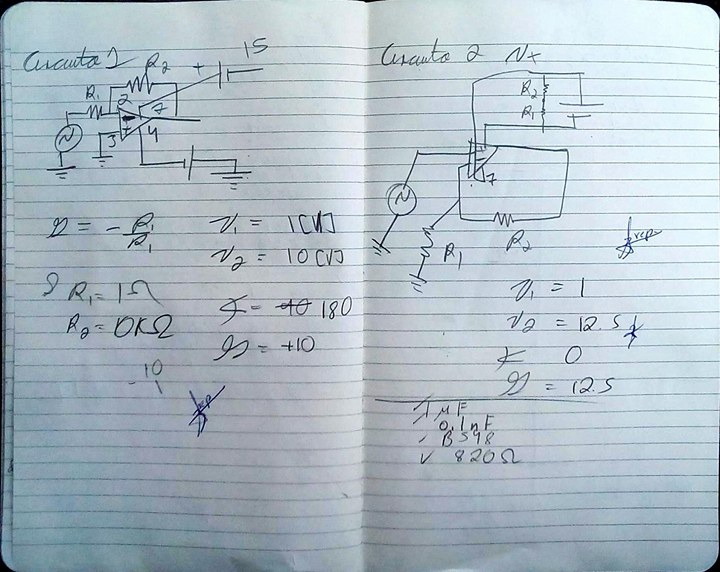
\includegraphics[scale=0.4]{OLensOpAmpBuffer.jpg}
    \caption{Circuitos realizados en el laboratorio}
    \label{fig:oLens}
\end{figure}

\section{Conclusiones}

Logramos apreciar el funcionamiento del Amplificador operacional como buffer, y sus diferencias en cuánto como es polarizado, esto es importante como características de diseño ya que el circuito es aparentemente equivalente pero se obtienen diferentes respuestas.



\bibliographystyle{plain}
\bibliography{Referencias}
\end{document}